\infolevone{
%\usepackage[small,scriptsize]{caption}
%\usepackage{fancyhdr}
%\newcommand{\Cerenkov}{\v{C}erenkov}
%\newcommand{\degrees}{$^\circ$}
%\newcommand{\NN}{$\mathrm{N_2}$}
%\newcommand{\CF}{$\mathrm{C_4F_{10}}$}
%\newcommand{\CO}{$\mathrm{CO_2}$}
%\newcommand{\OO}{$\mathrm{O_2}$}
%\newcommand{\MgF}{$\mathrm{MgF_2}$}
%\newcommand{\KCsSb}{$\mathrm{K_2CsSb}$}
%\newcommand{\GaP}{$\mathrm{GaP(Cs)}$}
%\newcommand{\dray}{$\delta\mathrm{-ray}$}
%\newcommand{\tr}[1]{\mathrm{Tr}\left\{#1\right\}}
%\newcommand{\Real}[1]{\mathrm{Re}\left\{#1\right\}}
%\newcommand{\Imag}[1]{\mathrm{Im}\left\{#1\right\}}
%\newcommand{\be}{\begin{enumerate}}
%\newcommand{\ee}{\end{enumerate}}
%\newcommand{\bi}{\begin{itemize}}
%\newcommand{\ei}{\end{itemize}}


%\pagestyle{fancy}
%\headheight 35pt


\subsection{Super HMS Noble Gas Cerenkov Detector}
Analyzing momenta up to 11~GeV/c at scattering angles from 5.5 to 40.0
degrees, the SHMS will reach kinematic regions in which the pion
background rate dominates the scattered electron rate by more than
1000:1.  The suppression of these anticipated pion backgrounds while
maintaining efficient identification of electrons is therefore one of
the main duties of the SHMS detector elements and the SHMS Noble Gas
\Cerenkov\ Detector shoulders a large portion of this particle
identification burden.  The design of the noble gas threshold \v
Cerenkov detector is such that it will meet these twin goals of
suppression and identification.  The main goal of the detector is to
distinguish between electrons and pions with momenta between 6 GeV and
11 GeV/c.

The basic equation  governing \v Cerenkov radiation emitted by a particle
of velocity $\beta$ traveling through a medium with index of refraction
$n$ is \begin{equation}\cos \theta = \frac{1}{\beta n},\end{equation}
where $\theta$ is the angle of the \v Cerenkov light cone.
From this it is easy to see that for there to be any radiation
$$n > 1/\beta.$$ What we need is that
\begin{equation} n < 1/\beta_{\pi,max}\label{eq:index} \end{equation}
to guarantee that the pions produce no radiation directly, and that
\begin{equation} n > 1/\beta_{e^-,min} \end{equation}
to guarantee that all the electrons produce Cerenkov light. Since
$1/\beta_{e^-,min} < 1/\beta_{\pi,max}$, we need to use only one value
of $n$ over the planned momentum range. Figure~\ref{fig:partsep}
emphasizes this point with a plot of the hadron velocity (given as
$(1-\beta)$) as a function of momentum along with the lines indicating
the index of refraction of various gases at 1 atm, as $(n-1)$.  For a
threshold Cerenkov counter only those particles with $(1-\beta) <
(n-1)$ will produce light. For example no $\pi$'s with momenta less
than 6 GeV/c will produce Cerenkov radiation in 1 ATM of Argon. If the
$\pi$'s momenta exceed 6 GeV/c then it will cross the `threshold' and
Cerenkov radiation will be emitted.
 \begin{figure}[!h] %  figure placement: here, top, bottom, or page
   \centering
   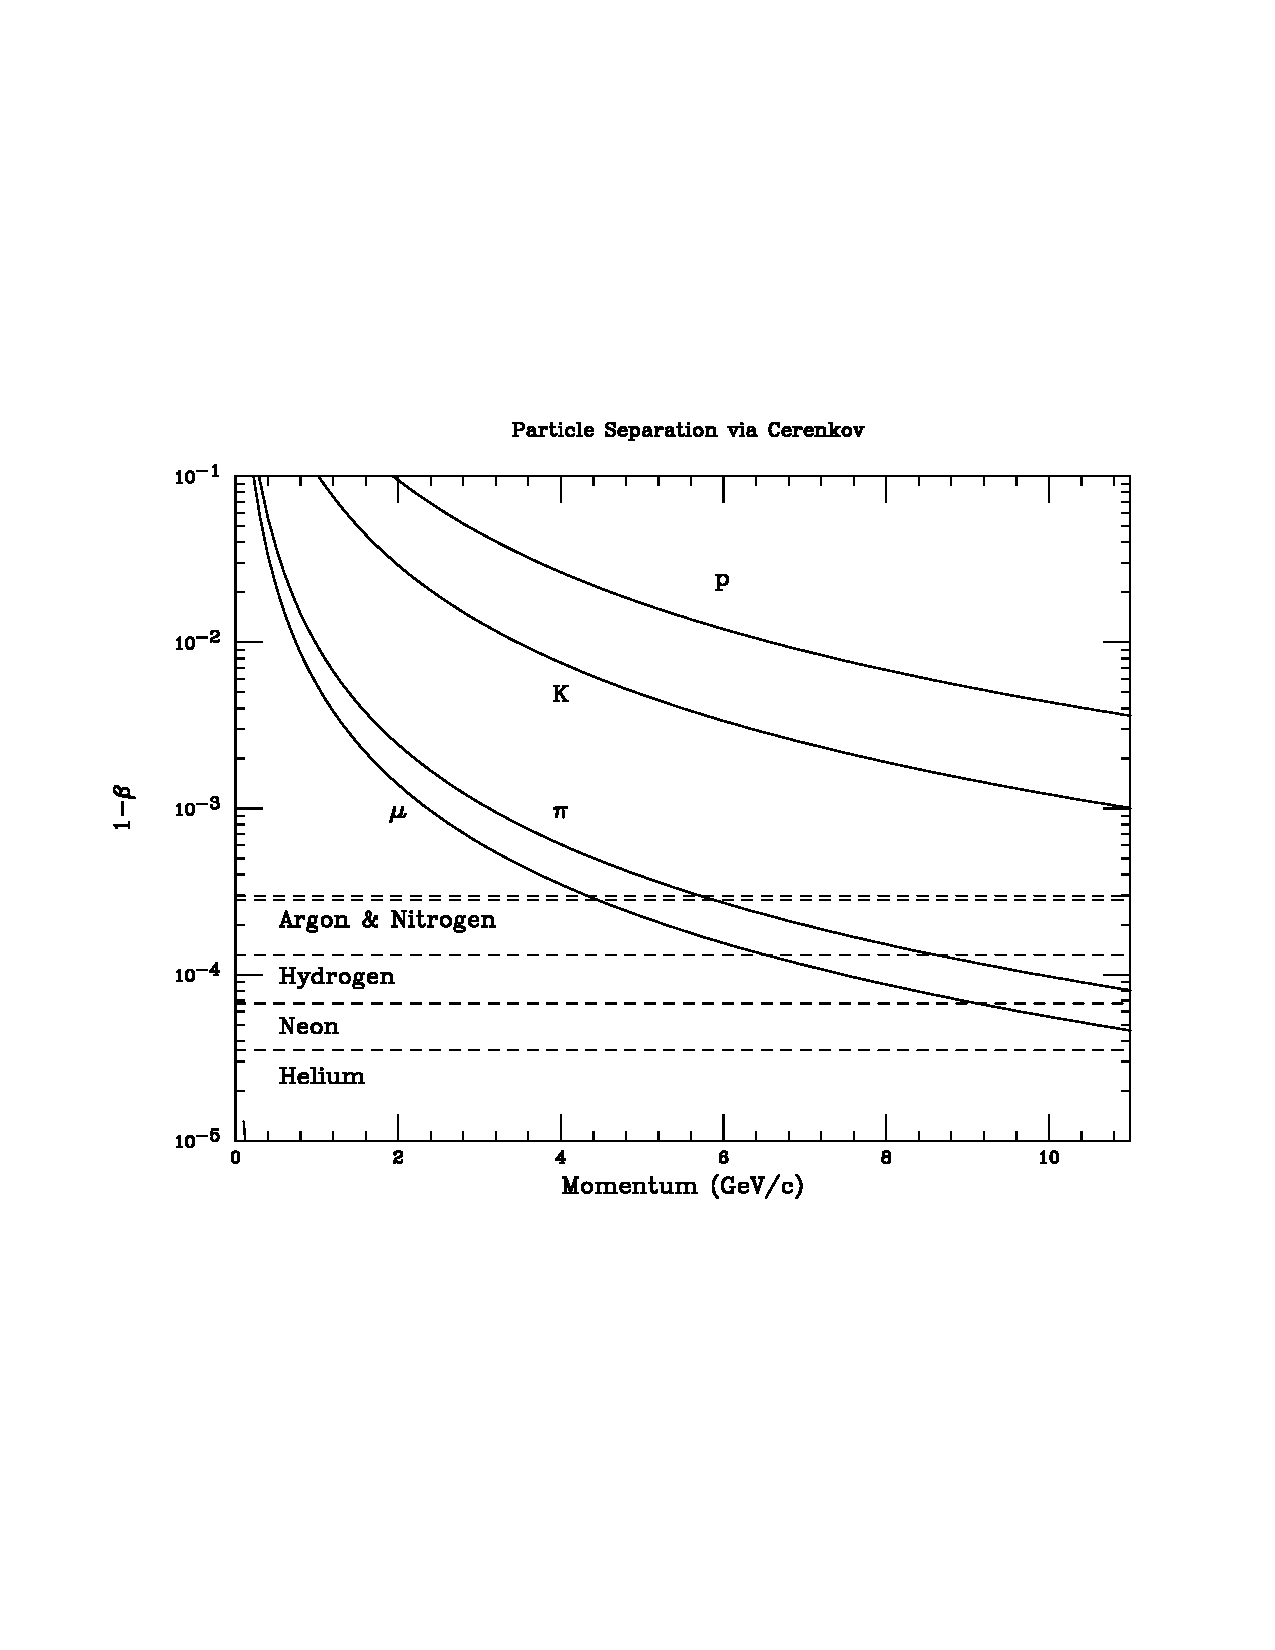
\includegraphics[width=0.8\textwidth]{ngc-partsep.pdf}
   \caption{Particle identification with a threshold Cerenkov
     detector. Plotted is the hadron velocity as $(1-\beta)$ against
     the hadron momenta. The horizontal lines indicate, for different
     gases at 1 ATM, the index of refraction as $(n-1)$. Only when
     $(1-\beta)$ is less than $(n-1)$ does the particle produce
     light.}
   \label{fig:partsep}
\end{figure}
A first glance at Fig.~\ref{fig:partsep} indicates that Neon would be
a good choice for the SHMS Cerenkov detector. Operation at 1 ATM allow
the windows on the detector tank to be very thin.

It is also possible to use a mixture of gases to fine tune the index
of refraction and improve the detector performance. In this case the
weighting of the index of refraction of the different gases is by the
number of molecules per unit volume for each gas and the index is
linear in the number per unit volume for each species. It should be
possible to obtain pre-mixed gases from a vendor or mix them using
techniques already in use at the laboratory. Hence the device has been
designed to use Argon and Neon at the limits of 6 GeV/c and 11 GeV/c
and a mixture in between.


The SHMS HGC design was restricted by the available space and the need
to have good discrimination at the highest momenta.  The number of
photoelectrons is maximized in this design by the use of quartz window
PMTs and mirrors with excellent reflectivity well into the UV. See
Fig.~\ref{fig:tubeandmirror}. It was also desired to have a minimum of
material in the path of the charged particles on order to keep
multiple scattering small and preserve the SHMS design
resolutions. The materials crossed by charged particles can be found
in Fig.~\ref{fig:materials}.

\newpage
\vspace{.25in}
\noindent {\bf Description of the Cerenkov}
\vspace{.25in}

The NGC consists of the following elements:
\begin{enumerate}
\item 2m long tank fabricated with an internal rigid frame and thin
  aluminum walls welded together. See Fig.~\ref{fig:Box}.

 The tank has an active volume of 2m along the beam direction and
 approximately 90 cm tank perpendicular to the beam direction. The
 tank was designed to position the PMTs outside the active area. The
 main access is provided through a large 'door' and four small panels
 provide modest access to the PMTS. There are large entrance and exit
 windows. The detector will operate at 1 ATM of either Argon or Neon
 or a mixture of the two. The tank has feed throughs for gas
 management as well as for HV and signal cables. A black flat paint
 has been applied to the interior of the tank to prevent the
 reflection of light from cosmic rays or hall background.

\item Four spherical thin glass mirrors of radius 135 cm, square in
  shape with edges of 43cm.

  The mirrors overlap in the center to provide full coverage of the
  active area and each focus the reflected Cerenkov light on a
  separate PMT. The mirrors are tilted by 15$^\circ$ to allow the PMTs
  to be outside he active area.  The mirrors are positioned in a
  monolithic frame that is installed as single unit. The mirrors are
  installed, the overlap set and rotated with the frame on a table
  outside the tank.  See~Fig.\ref{fig:install}.
\item Four 14~stage 5~inch quartz window PMTs manufactured by Electron
  Tubes Enterprises.

 The PMTs are model 9823QKB04 and tubes with serial numbers 16747,
 16777, 16787 and 16785 are installed to accept light from the mirrors
 in position Top Right, Top Left, Bottom Right and Bottom Left
 respectively while looking along increasing $z$. The tubes are
 surrounded by a mu-metal shield and the HV is distributed to the
 stages by a positive base.
\item Thin entrance and exit window made of two layers of 2 mils of
  the Dupont product, Tedlar - (CH$_2$CHCl)$_n$.
\end{enumerate}
\begin{figure}[!h] %  figure placement: here, top, bottom, or page
   \centering
   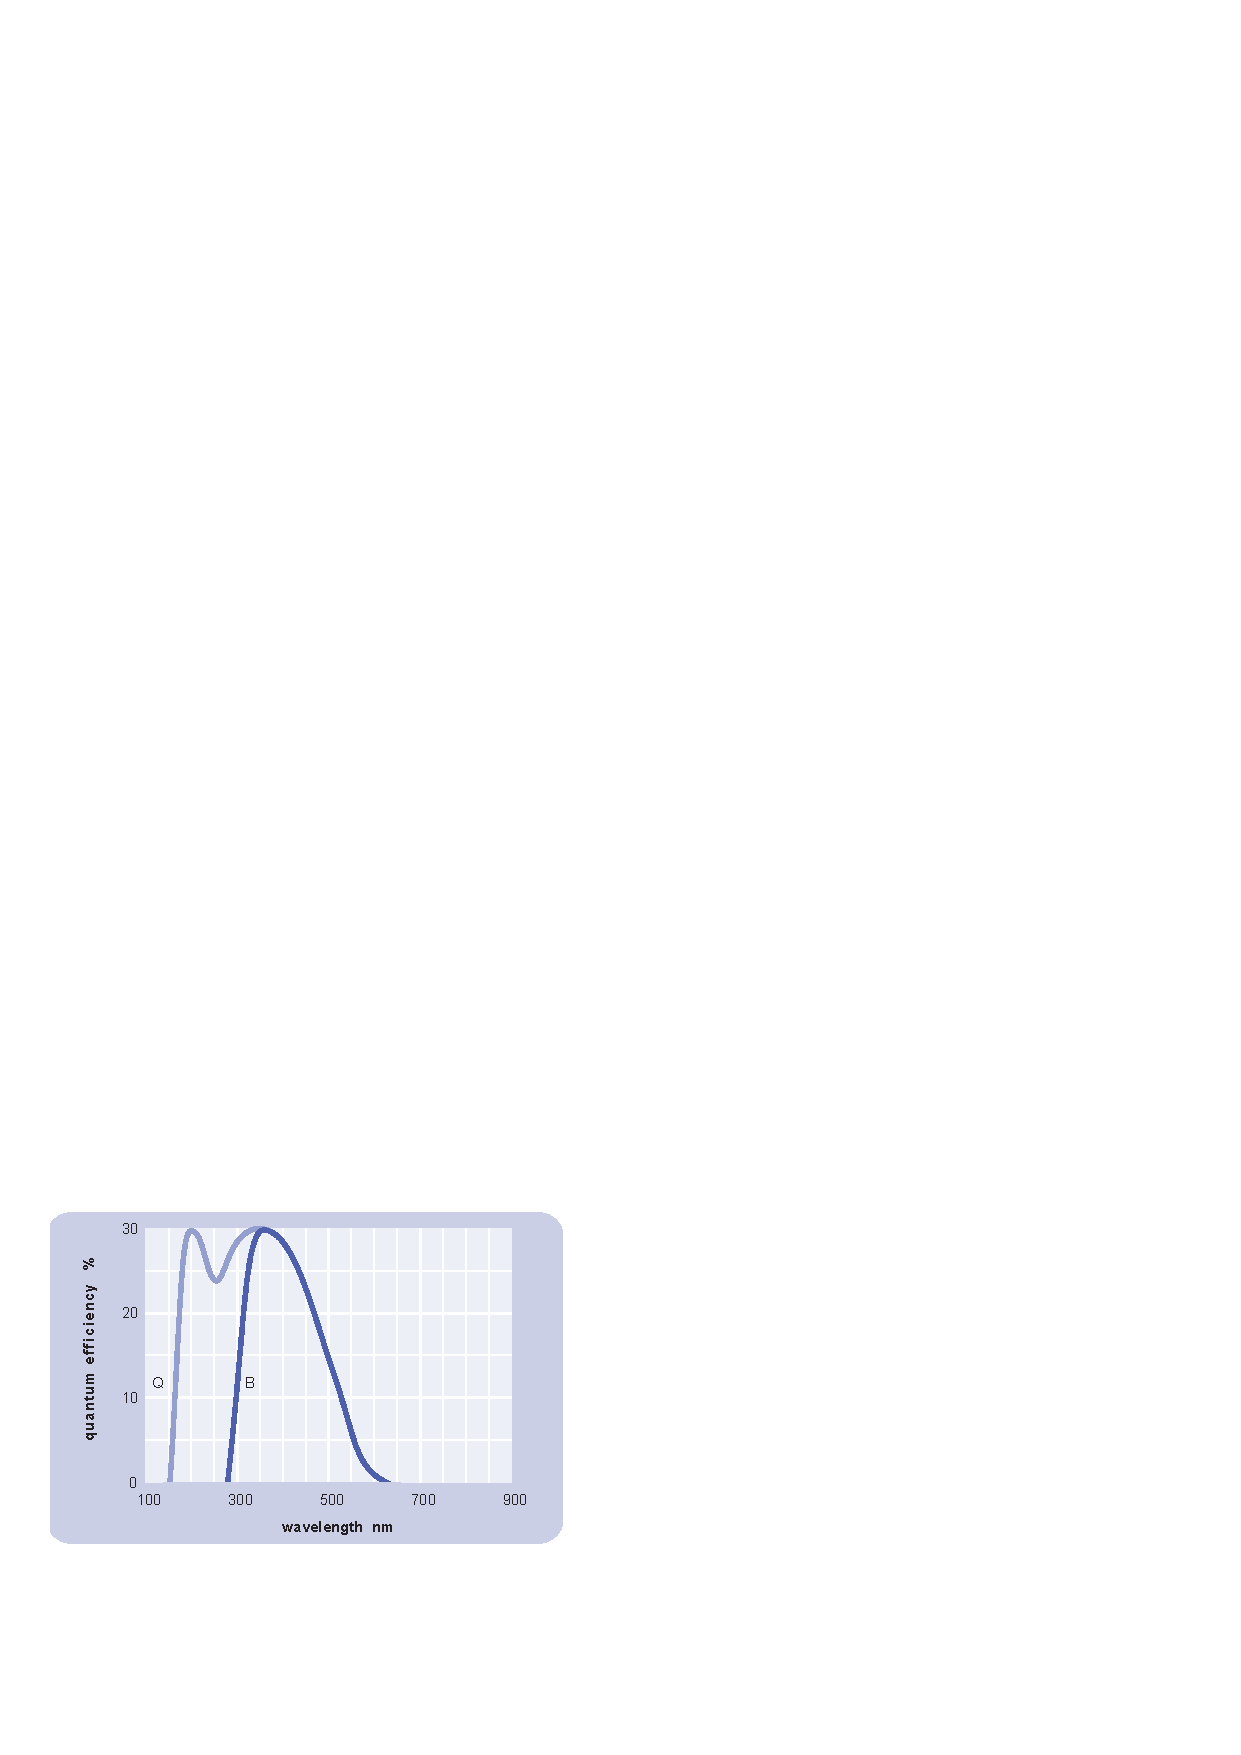
\includegraphics[width=.45\textwidth]{ngc-9832BQ.pdf}
   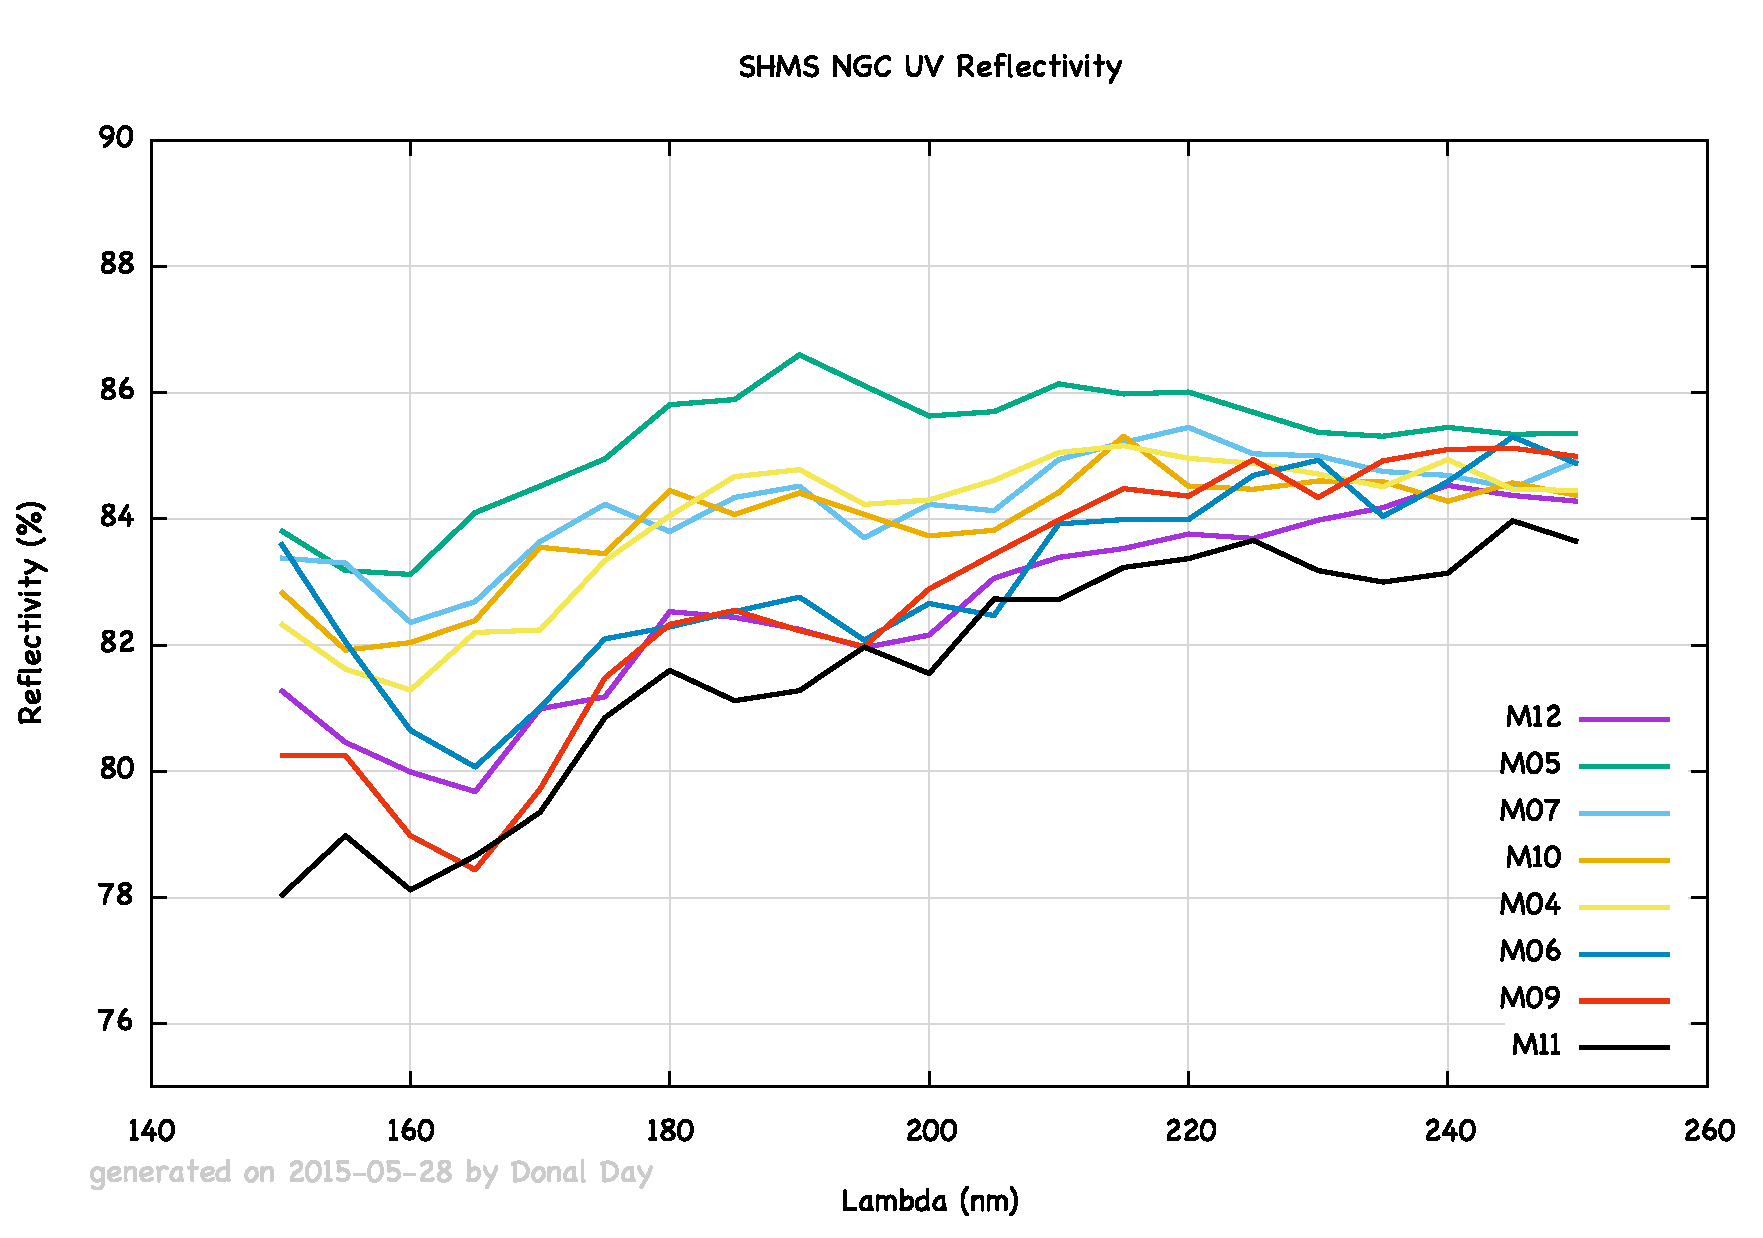
\includegraphics[width=.45\textwidth]{ngc-UVReflectanceCERN.pdf}
   \caption{LHS:
     Quantum efficiency of Electron Tubes Enterprises model 9823QKB04
     - light blue curve, labelled ``Q". RHS: The UV measured
     reflectivity of the mirrors coated at CERN. Between 250 nm and
     600 nm the reflectivity rises to almost
     90\%. \label{fig:tubeandmirror}}

\end{figure}
\begin{figure}[!h] %  figure placement: here, top, bottom, or page
   \centering
   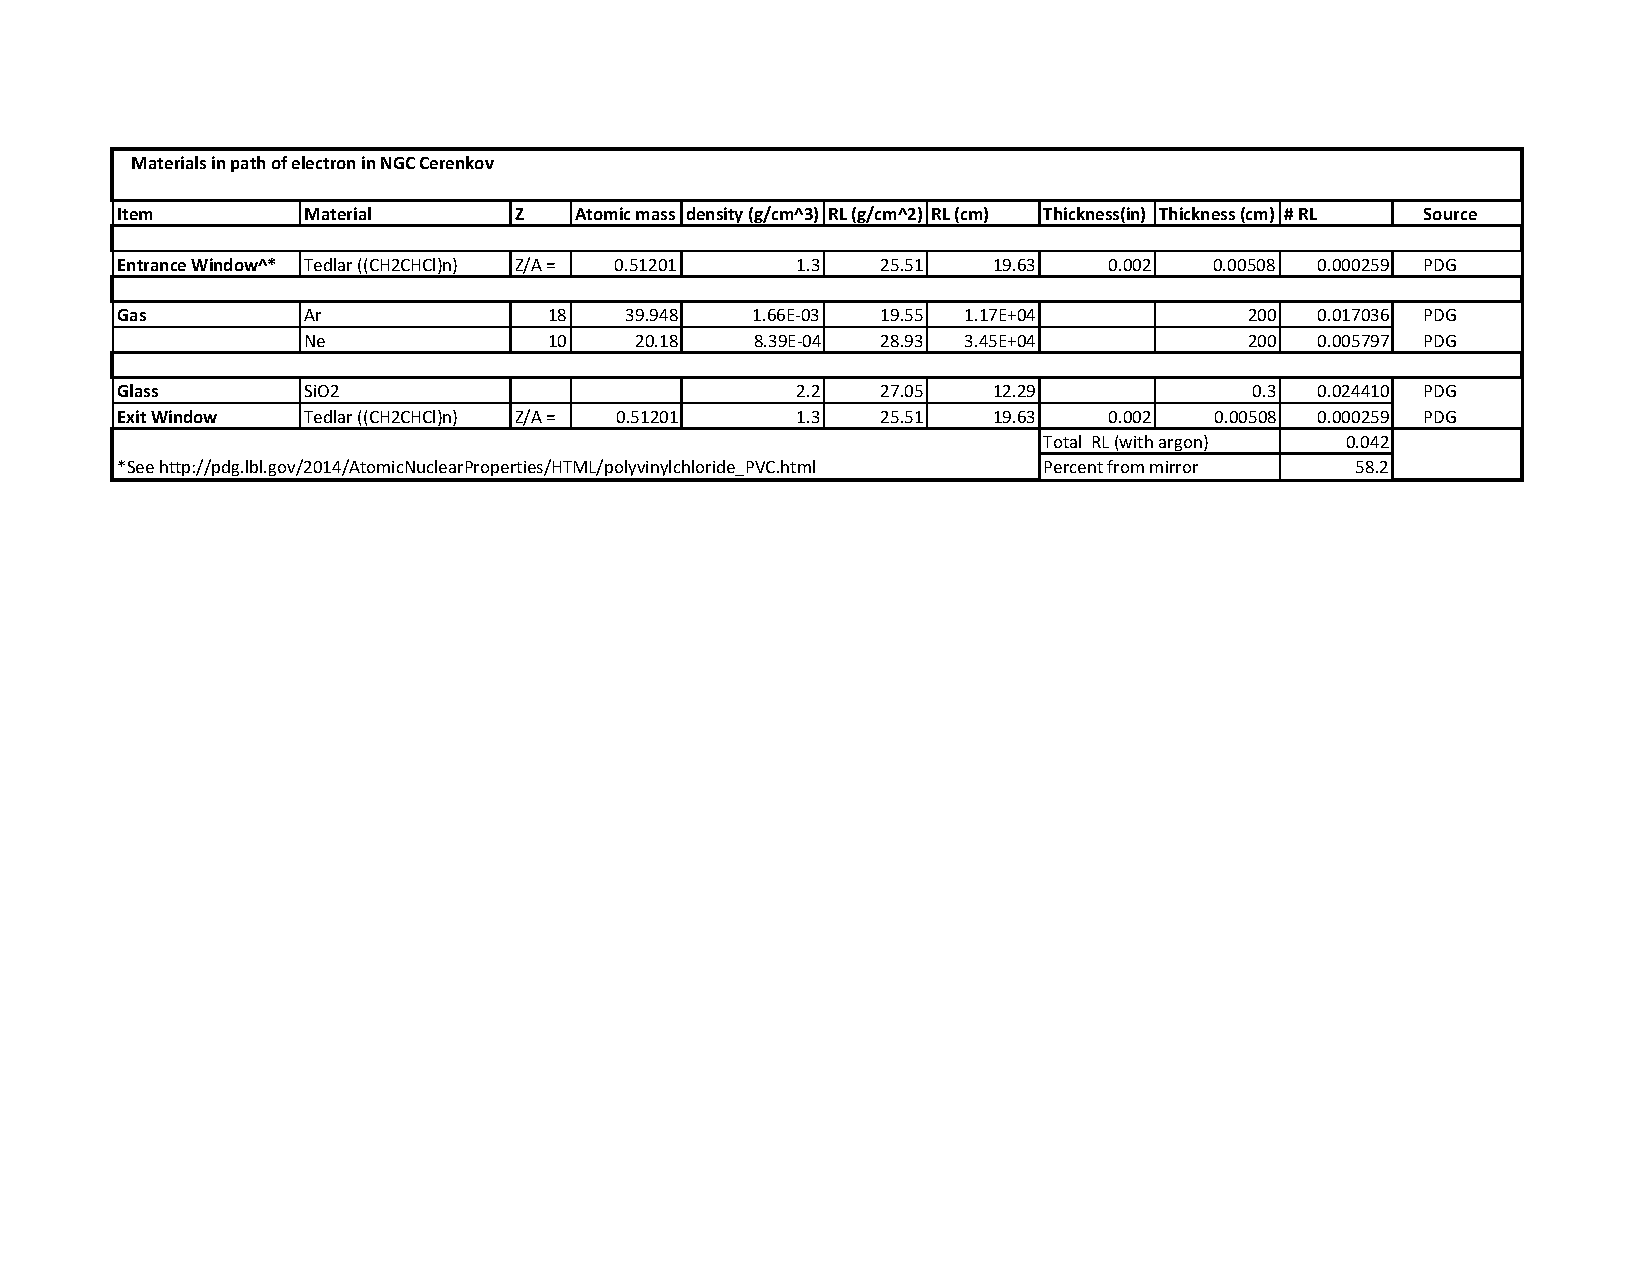
\includegraphics[width=\textwidth]{ngc-MaterialsinCerenkovFeb2016Crop.pdf}
   \caption{Materials
     in the path of charged particles passing through the
     NGC.\label{fig:materials}}
\end{figure}



\begin{figure}[!h] %  figure placement: here, top, bottom, or page
   \centering
   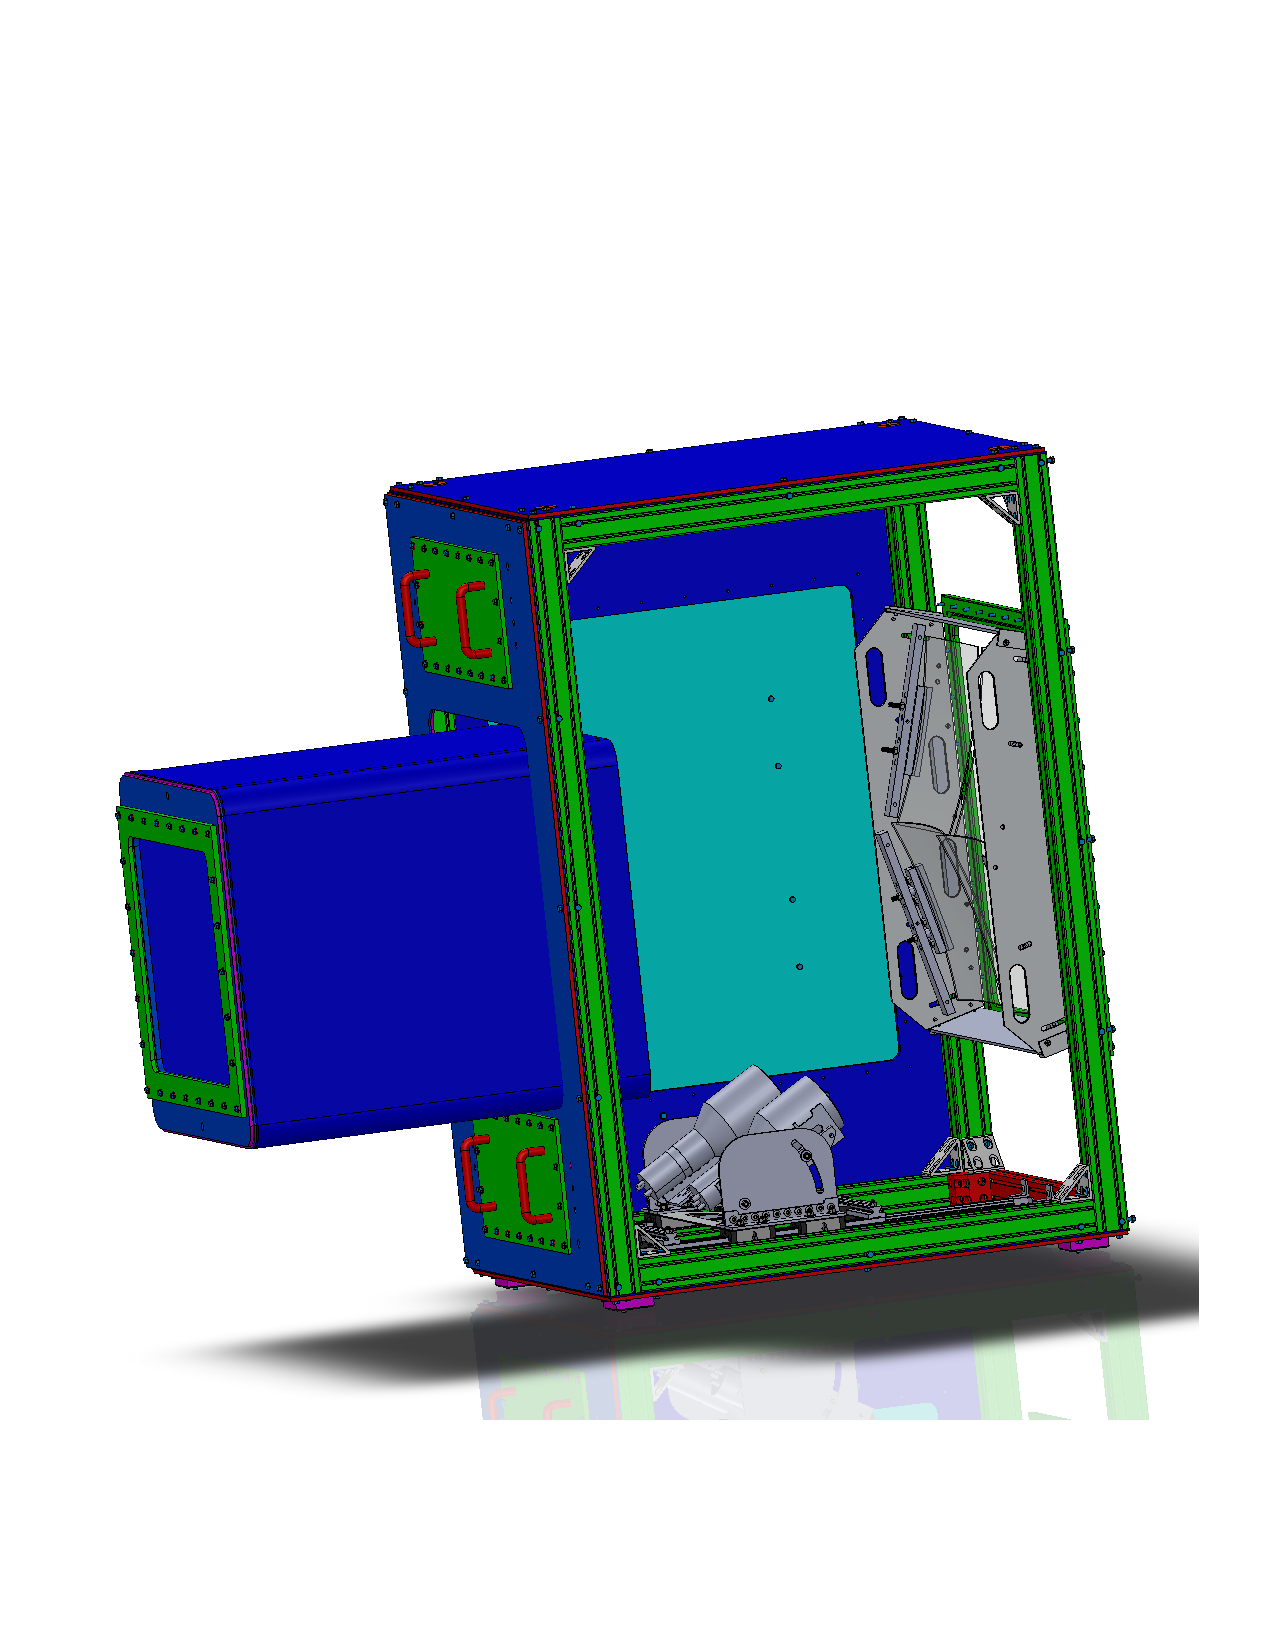
\includegraphics[width=0.45\textwidth]{ngc-fullconstruction.pdf}
   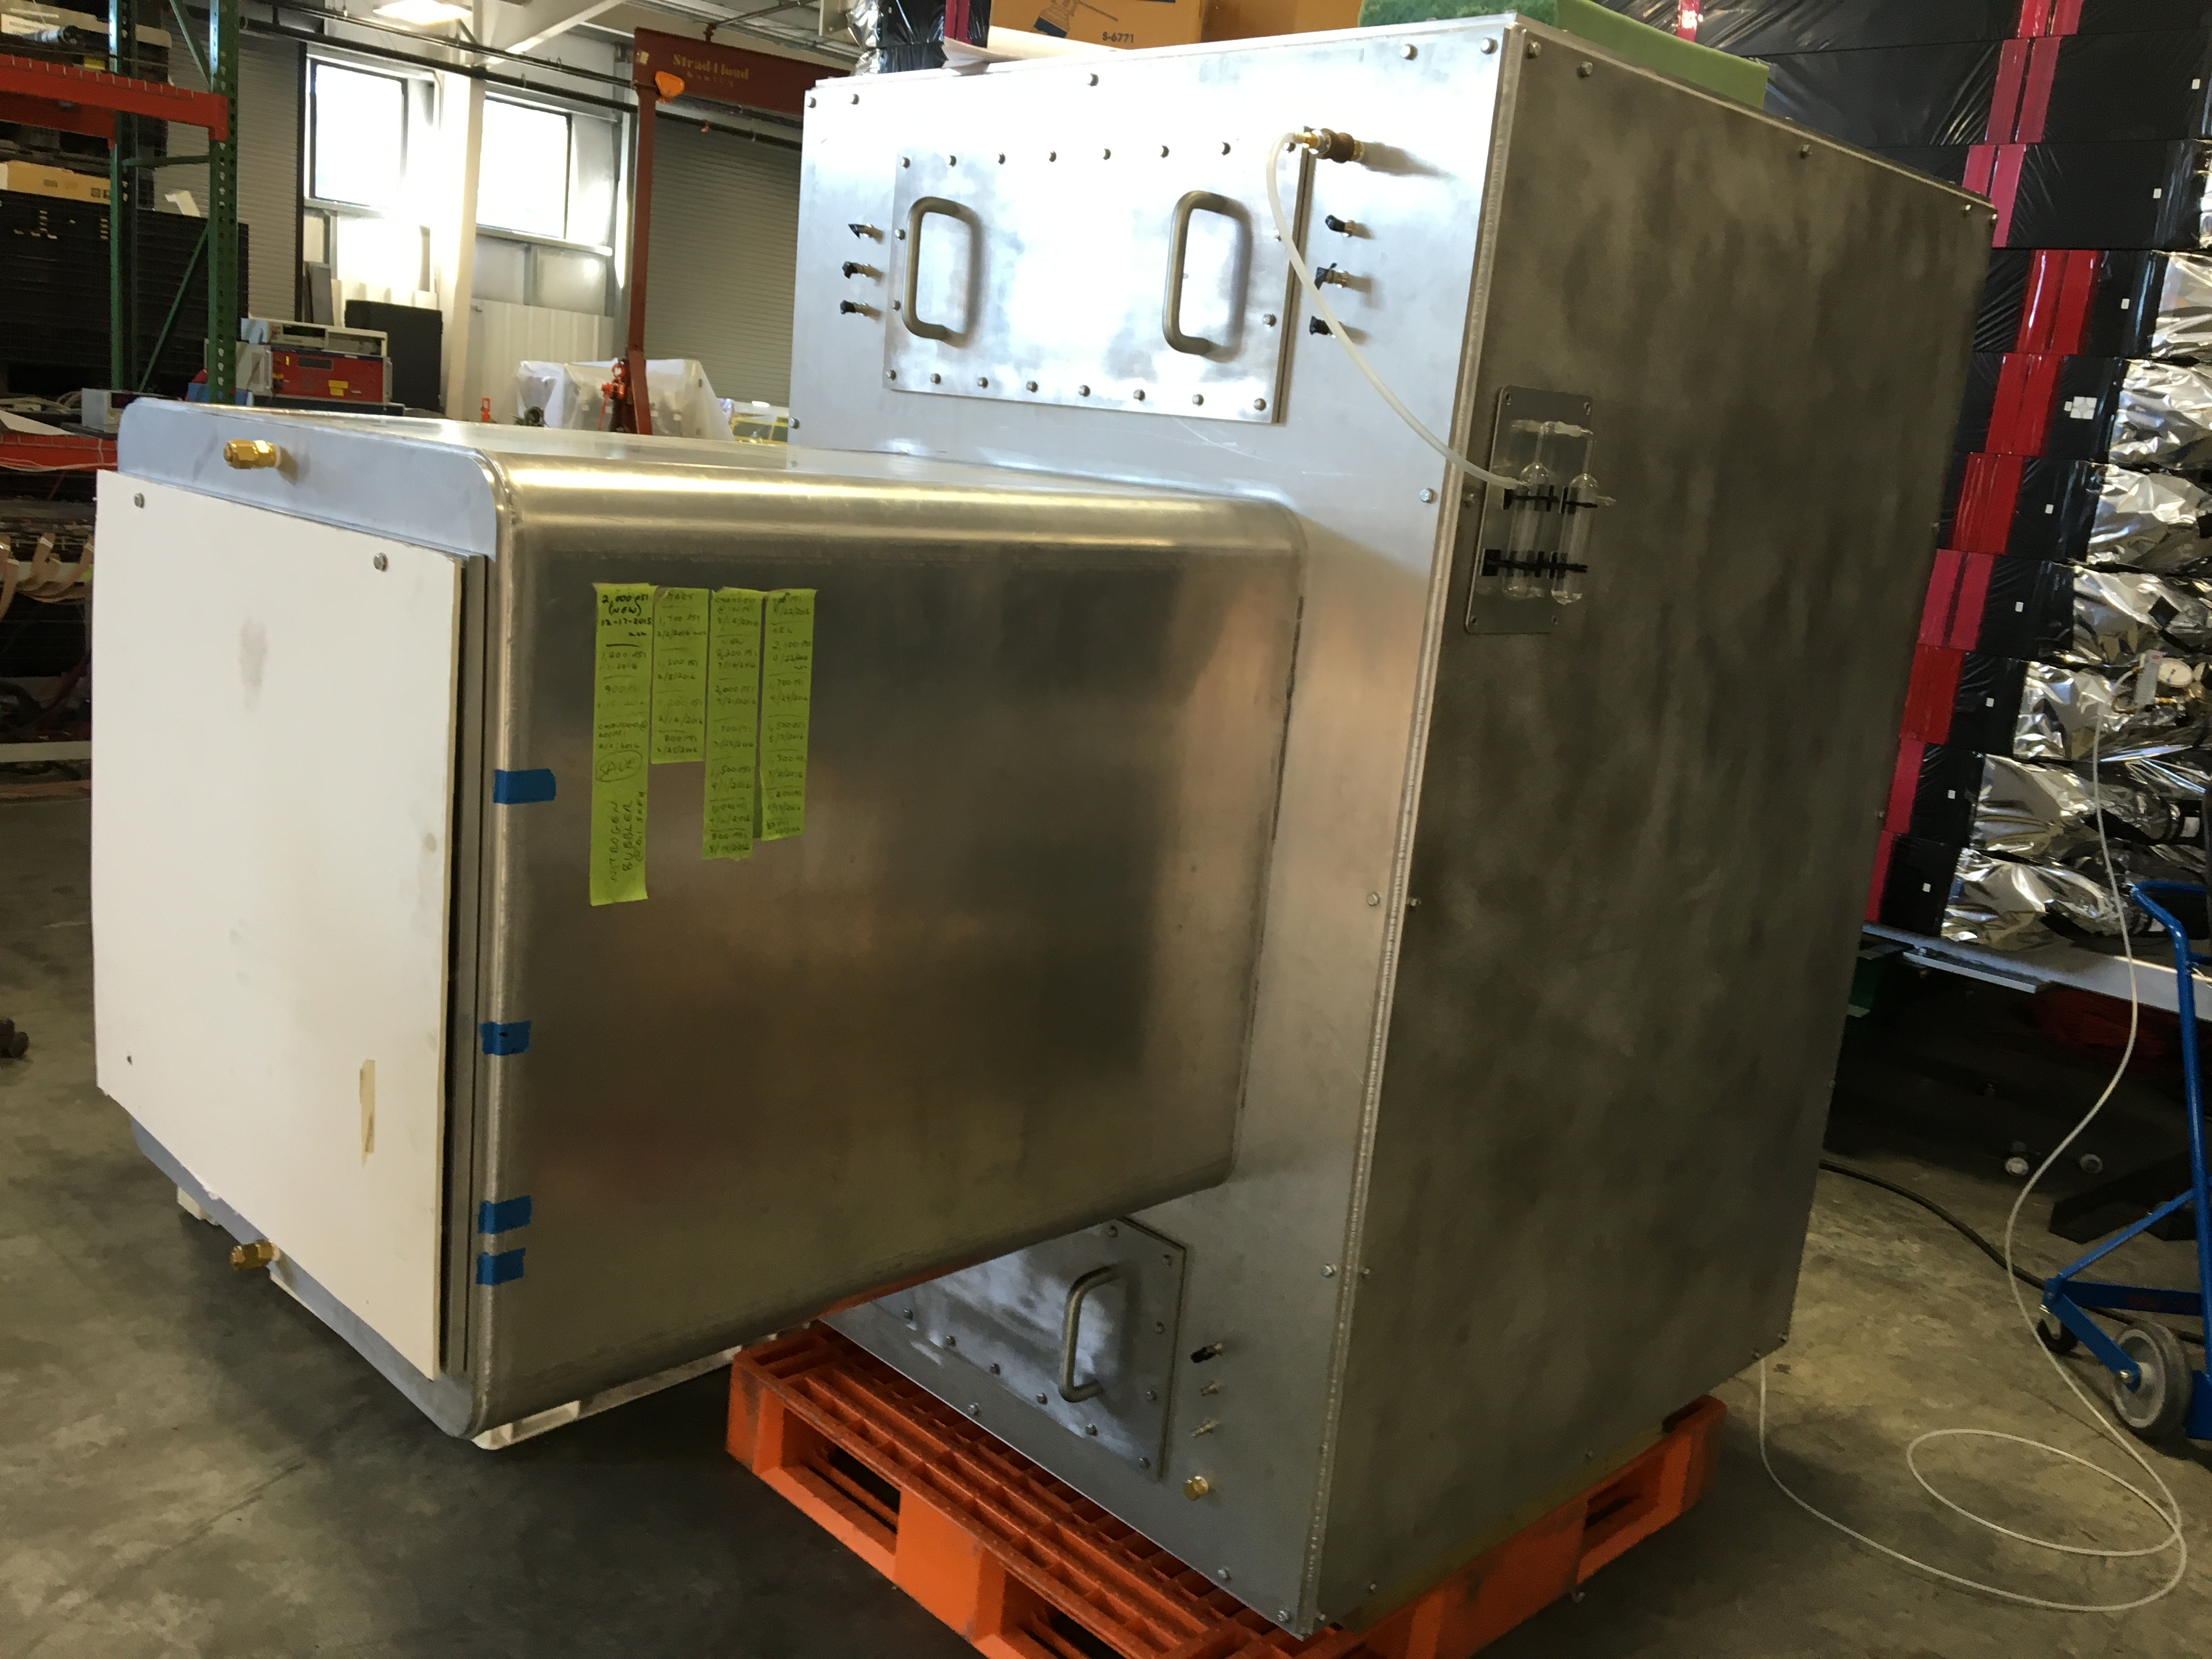
\includegraphics[width=0.45\textwidth]{ngc-TankAsBuilt.jpg}
   \caption{LHS: Sketch of the NGC tank. This view is possible as one
     panel is removed. Note the PMT mounting system is different than
     shown here.  RHS: Buttoned up tank waiting
     installation.\label{fig:Box}}

\end{figure}

%\vspace{.25in}
%\noindent {\bf{Gas Filling Procedure - to be added}}  % BDS TODO
%\vspace{.25in}

The tank contains four 5 inch PMT's which use {\bf positive} HV. They
operate at between 1900 and 2400 Volts. The Anode is at HV and its
signal is viewed through a decoupling capacitor in the base.  The
HV is supplied via the Hall C High Voltage system (see
section~\ref{sec:highvoltage}).

The mirrors in the tank may require adjustment for optimal focusing on
the PMT faces. This is only possible when the tank is out of the SHMS
and on a horizontal surface (the hall floor) and the access door
removed allowing entry into the tank. The tank is a confined space and
hence this activity represents an ODH ha zard. Stickers indicating this
have been placed on the PMT ports and on the door. Before an entry
into the tank the atmosphere in the interior must be surveyed by a
member of the physics division EH$\&$S staff.  This adjustment should
only be done by personnel with experience. A document, ``NGC Mirror
Installation and Tuning'', has been written describing the optical
tuning and it can be found at
\url{https://hallcweb.jlab.org/doc-private/ShowDocument?docid=794}

\begin{figure}[!h] %  figure placement: here, top, bottom, or page
   \centering
   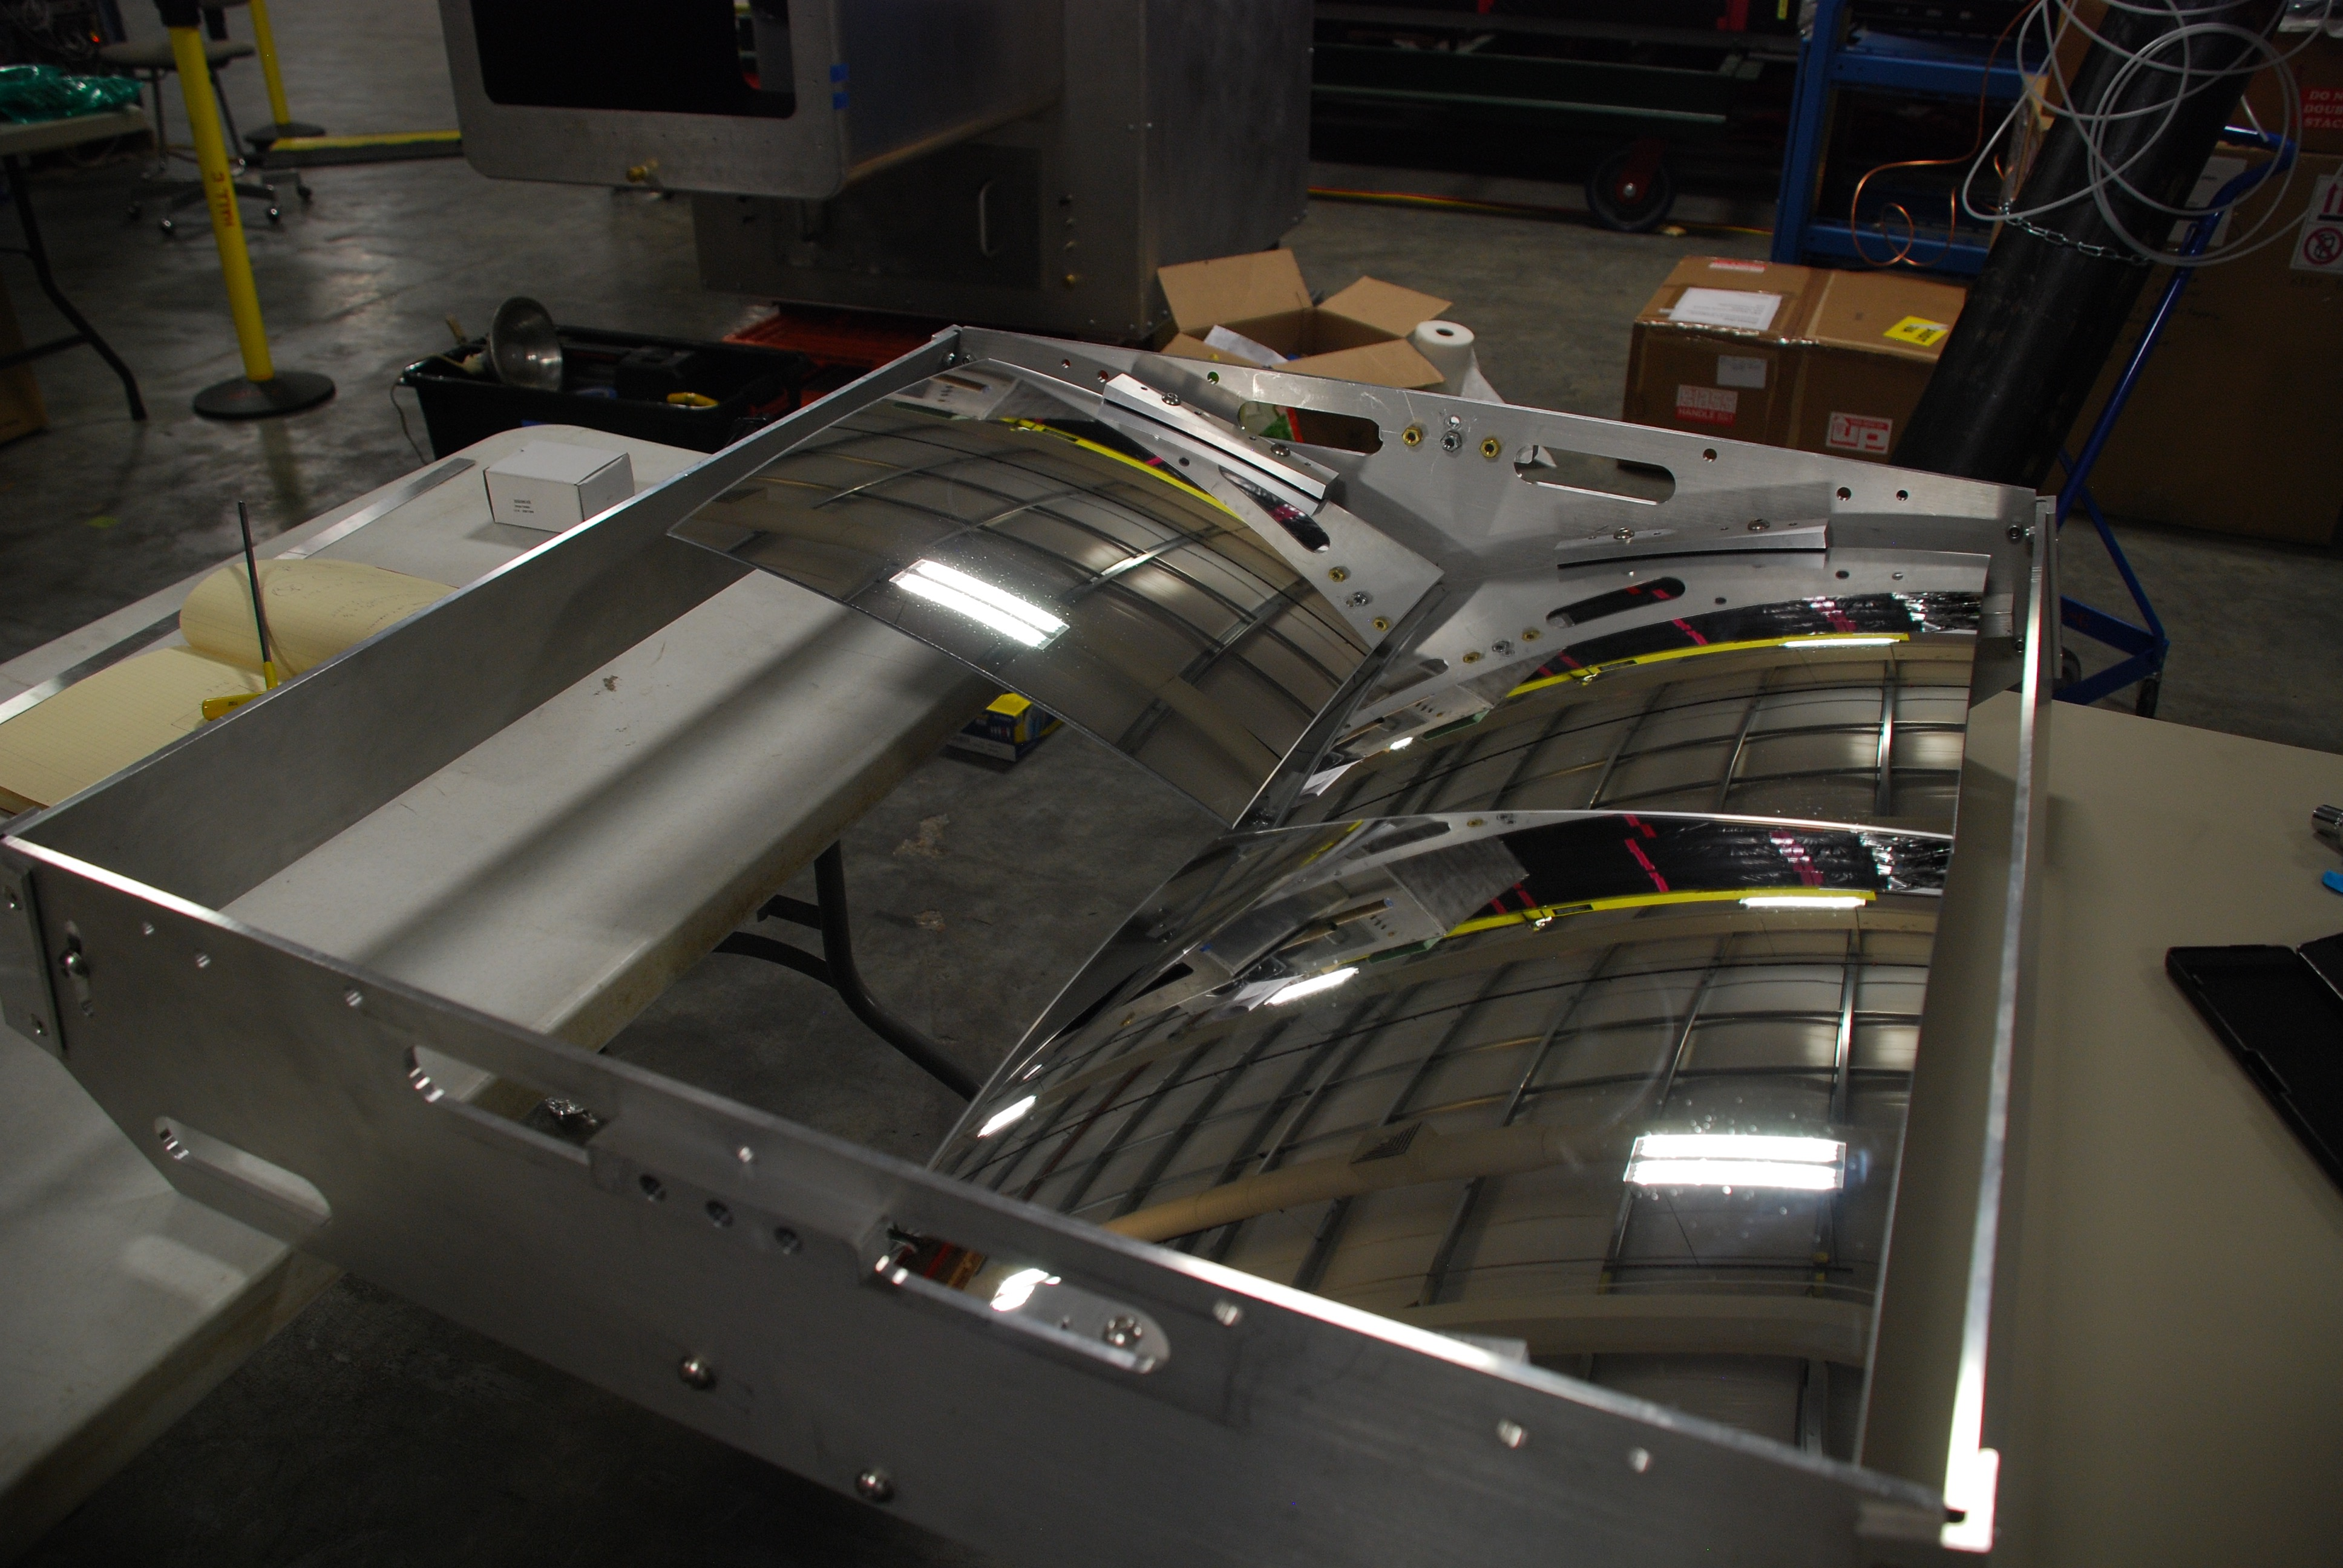
\includegraphics[width=0.45\textwidth]{ngc-TwoMirrorsinFrame.jpg}
   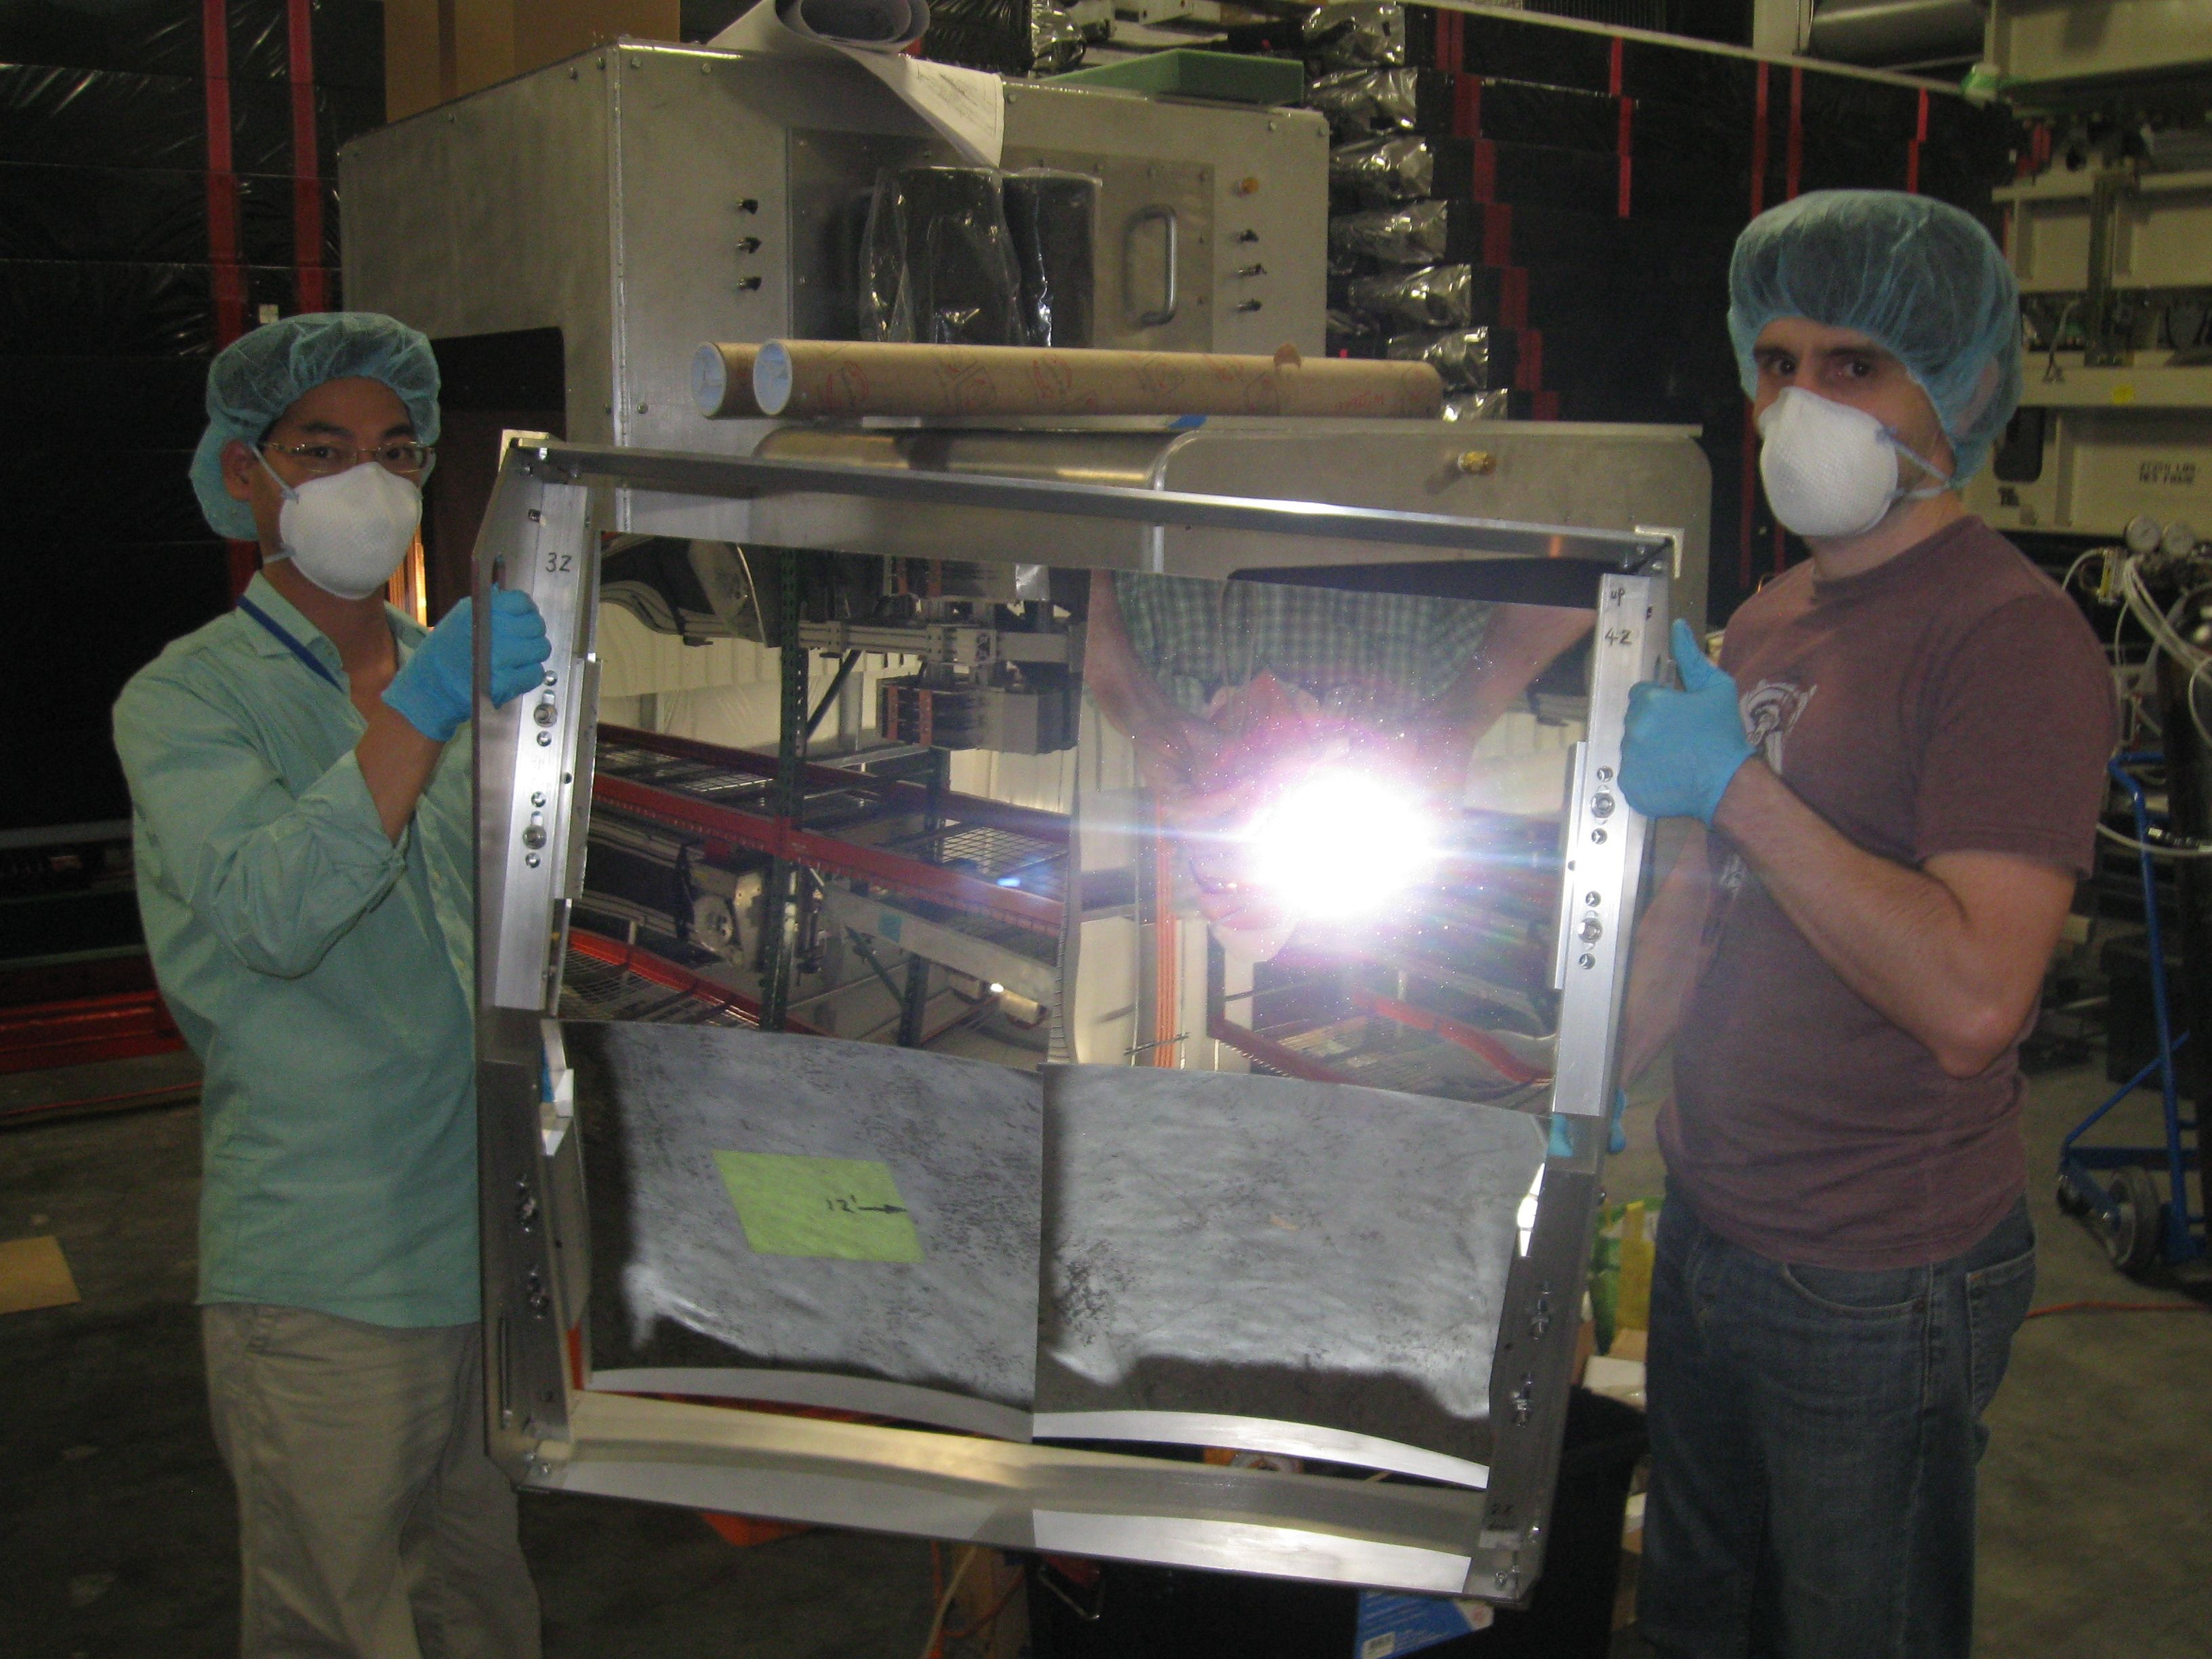
\includegraphics[width=0.45\textwidth]{ngc-GoingIn.jpg}
   \caption{LHS: Three of four mirrors installed in frame. RHS: Frame
     about to be moved into tank.\label{fig:install}}

   \end{figure}
}% \infolevone
